\documentclass{beamer}
\definecolor{iclblue}{RGB}{0, 62, 116}
\definecolor{iclnavy}{RGB}{0, 33, 71}
\usepackage{xcolor}
\usepackage{caption}

\mode<presentation>{
\usetheme{default}
\usecolortheme{default}
\usefonttheme{structurebold}
\setbeamertemplate{navigation symbols}{}
\setbeamertemplate{caption}[numbered]

%\setbeamercolor{palette primary}{fg = white, bg = iclblue}
%\setbeamercolor{palette secondary}{fg = white, bg = iclblue}
%\setbeamercolor{palette tertiary}{fg = white, bg = iclblue}
%\setbeamercolor{palette quaternary}{fg = white, bg = iclblue}

\setbeamercolor{title}{fg = iclblue}
\setbeamercolor{structure}{fg = iclblue}
\setbeamercolor{section in toc}{fg = iclblue}

\setbeamercolor{frametitle-left}{fg=iclblue}
\setbeamercolor{frametitle}{fg=iclblue}
\setbeamerfont{frametitle}{size=\LARGE\bfseries\vspace{0.2cm}}
}

\usepackage[english]{babel}
\usepackage[utf8]{inputenc}
\usepackage[T1]{fontenc}

\logo{\includegraphics[width = 0.4\textwidth]{../Images/icllogo.jpg}}

\title{\textbf{Climactic Drivers of Mosquito Abundance}}
\author{Anne Marie Saunders}
\institute{MSc Computational Methods in Ecology and Evolution \\ Imperial College London \\ \vspace{0.5cm} Supervisors: \\ Samraat Pawar, Lauren Cator, Ruiyun Li, Matthew Watts}
\date{April 31, 2020}

\begin{document}

\begin{frame}
	\titlepage
\end{frame}

\begin{frame}{}
\frametitle{Outline}

		%\tableofcontents
		
		\bfseries Introduction \\ \vspace{0.2cm}
		Research Questions \\ \vspace{0.2cm}
		Data \\ \vspace{0.2cm}
		Methods \\ \vspace{0.2cm}
		Progress \\ \vspace{0.2cm}
		Next Steps \\ \vspace{0.2cm}
		Questions
		

\end{frame}

\section{Introduction}

\begin{frame}
\frametitle{Introduction}
\begin{itemize}
	\item Mosquitoes are vectors of many human diseases \textcolor{white}{
	\item Being able to predict abundances can help optimize control measures
	\item Abundance dynamics are dependent on environmental factors that are likely to be affected by climate change}
	
	\includegraphics[width= 0.6\textwidth]{../Images/wnv_cases.pdf}
\end{itemize}

\end{frame}

\begin{frame}{}
\frametitle{Introduction}
\begin{itemize}
	\item Mosquitoes are vectors of many human diseases 
		\item The ability to predict changes in abundance could help optimize control measures\textcolor{white}{
		\item Abundance dynamics are dependent on environmental factors that are likely to be affected by climate change}
	
	\includegraphics[width= 0.6\textwidth]{../Images/wnv_cases.pdf}
\end{itemize}

\end{frame}

\begin{frame}{}
\frametitle{Introduction}
\begin{itemize}
	\item Mosquitoes are vectors of many human diseases 
	\item The ability to predict changes in abundance could help optimize control measures
	\item Abundance dynamics are dependent on environmental factors that are likely to be affected by climate change
	
	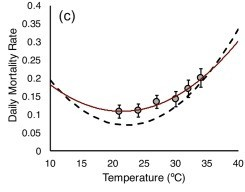
\includegraphics[width= 0.6\textwidth]{../Images/tpc.jpg}
	
	\footnotesize Adapted from Shapiro et al. 2017
	
\end{itemize}

\end{frame}

\section{Questions}
\begin{frame}
\frametitle{Questions}

\begin{enumerate}\Large
	\item Which length of temporal lag of meteorological variables is most appropriate for estimating mosquito abundance dynamics? \vspace{.3cm}
	
	\item \textcolor{white}{Which temporal scale of environmental drivers best predicts mosquito abundance changes?} \vspace{.3cm}
	
	\item \textcolor{white}{Can a model developed from these questions predict West Nile Virus risk?}
	\vspace{1cm}
	
\end{enumerate}

\end{frame}


\begin{frame}
\frametitle{Questions}

\begin{enumerate}\Large
\item Which length of temporal lag of meteorological variables is most appropriate for estimating mosquito abundance dynamics? \vspace{.3cm}

	\item Which temporal scale of environmental drivers best predicts mosquito abundance changes? \vspace{.3cm}
	\textcolor{white}{
	\item Can a model developed from these questions predict West Nile Virus risk?}
\vspace{1cm}

\end{enumerate}

\end{frame}

\begin{frame}
\frametitle{Questions}

\begin{enumerate}\Large
	\item Which length of temporal lag of meteorological variables is most appropriate for estimating mosquito abundance dynamics? \vspace{.3cm}
	
	\item Which temporal scale of environmental drivers best predicts mosquito abundance changes? \vspace{.3cm}
	
	\item Can a model developed from these questions predict West Nile Virus risk?
	\vspace{1cm}
	
\end{enumerate}

\end{frame}

\section{Data}

\begin{frame}{}
\frametitle{Data}
\begin{columns}
	\begin{column}{0.5\textwidth}
		\begin{itemize}
			\item VectDyn: 206 datasets worldwide
			\item 7 Florida counties, 5 of which have high quality datasets
			\item Climate data from NOAA
		\end{itemize}
	\vspace{1cm}
	\end{column}
	\begin{column}{0.5\textwidth}  %%<--- here
		\begin{center}
			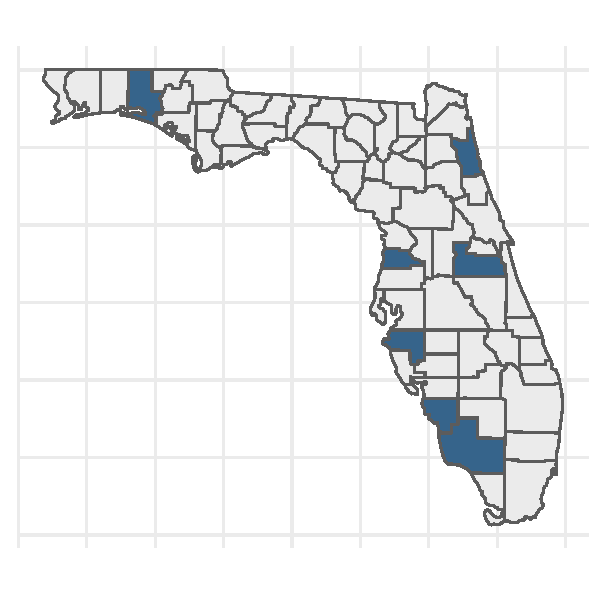
\includegraphics[height = 4.5cm, width=.9\textwidth]{../Images/floridamap.pdf}
		\end{center}
	\vspace{1cm}
	\end{column}
\end{columns}
	
\end{frame}

\section{Methods}

\begin{frame}{}
	\frametitle{Methods}
	
	\begin{enumerate}
		\item Extract Florida abundance datasets from large raw data file 
		
		\item Extract climate data from NOAA temperature and precipitation rasters and map to abundance data
		
		\item Aggregate datasets to weekly, biweekly, and monthly scales to create time series
		
		\item \textcolor{white}{Fit time series models with a range of temporal lags at different time scales}
		
		\item \textcolor{white}{Conduct model selection}
		
		\item \textcolor{white}{Use SIR models with abundance incorporated to transmission rate to estimate disease risk}
		
		\item \textcolor{white}{Compare to disease surveillance data}
		
	\end{enumerate}
	
\end{frame}

\begin{frame}{}
\frametitle{Methods}

\begin{enumerate}
	\item Extract Florida abundance datasets from large raw data file 
	
	\item Extract climate data from NOAA temperature and precipitation rasters and map to abundance data
	
	\item Aggregate datasets to weekly, biweekly, and monthly scales to create time series
	
	\item Fit time series models with a range of temporal lags at different time scales
	
	\item Conduct model selection 
	
	\item Use SIR models with abundance incorporated to transmission rate to estimate disease risk
	
	\item Compare to disease surveillance data
	
\end{enumerate}

\end{frame}

\section{Progress}

\begin{frame}
\frametitle{Extraction}

\begin{enumerate}
	\item Extract Florida abundance datasets 
	
	\item Extract climate data 
	
	\item Aggregate to weekly, biweekly, and monthly scales	
\end{enumerate}
	

\vspace{0.7cm}
\begin{columns}
	\begin{column}{0.7\textwidth}
		\includegraphics[width = \textwidth]{../Images/temp_extracted.pdf}
	\end{column}
	\begin{column}{0.3\textwidth}
		
	\end{column}
\end{columns}

\end{frame}

\begin{frame}
\frametitle{Extraction}

\begin{enumerate}
	\item Extract Florida abundance datasets 
	
	\item Extract climate data 
	
	\item Aggregate to weekly, biweekly, and monthly scales	
\end{enumerate}


\vspace{0.7cm}
\begin{columns}
	\begin{column}{0.7\textwidth}
		\includegraphics[width = \textwidth]{../Images/count_extracted.pdf}
	\end{column}
	\begin{column}{0.3\textwidth}
		
	\end{column}
\end{columns}

\end{frame}

\begin{frame}
\frametitle{Aggregation}

\begin{enumerate}
	\item Extract Florida abundance datasets 
	
	\item Extract climate data 
	
	\item Aggregate to weekly, biweekly, and monthly scales	
\end{enumerate}


\vspace{0.7cm}
\begin{columns}
	\begin{column}{0.7\textwidth}
		\includegraphics[width = \textwidth]{../Images/weekly_agg.pdf}
	\end{column}
	\begin{column}{0.3\textwidth}
		
	\end{column}
\end{columns}

\end{frame}

\begin{frame}
\frametitle{Aggregation}

\begin{enumerate}
	\item Extract Florida abundance datasets 
	
	\item Extract climate data 
	
	\item Aggregate to weekly, biweekly, and monthly scales	
\end{enumerate}


\vspace{0.7cm}
\begin{columns}
	\begin{column}{0.7\textwidth}
		\includegraphics[width = \textwidth]{../Images/biweekly_agg.pdf}
	\end{column}
	\begin{column}{0.3\textwidth}
		
	\end{column}
\end{columns}

\end{frame}


\begin{frame}
\frametitle{Aggregation}

\begin{enumerate}
	\item Extract Florida abundance datasets 
	
	\item Extract climate data 
	
	\item Aggregate to weekly, biweekly, and monthly scales	
\end{enumerate}


\vspace{0.7cm}
\begin{columns}
	\begin{column}{0.7\textwidth}
		\includegraphics[width = \textwidth]{../Images/monthly_agg.pdf}
	\end{column}
	\begin{column}{0.3\textwidth}
		
	\end{column}
\end{columns}

\end{frame}

\section{Next Steps}

\begin{frame}
\frametitle{Model Fit and Selection}

\begin{enumerate}
	\setcounter{enumi}{3}
	\item Fit time series models: vary time scales and temporal lags using GLM, GAM, or ZIGAM
	
	\item Model selection: AIC/BIC/Likelihood Ratio Test
	
\end{enumerate}
\vspace{0.1cm}
\small
General Model Format:
$$ Abundance_t = Temperature_{t-lag} + Precipitation_{t-lag} $$
\textcolor{white}{
Generalized Linear Model:
$$ M_t = a_1T_{t-lag}^2 + a_2T_{t-lag} + b_1P_{t-lag}^2 + b_2P_{t-lag} + c$$
}
\end{frame}


\begin{frame}
\frametitle{Model Fit and Selection}

\begin{enumerate}
	\setcounter{enumi}{3}
	\item Fit time series models: vary time scales and temporal lags using GLM, GAM, or ZIGAM
	
	\item Model selection: AIC/BIC/Likelihood Ratio Test
	
\end{enumerate}
\vspace{0.1cm}
\small
General Model Format:
$$ Abundance_t = Temperature_{t-lag} + Precipitation_{t-lag} $$

Generalized Linear Model:
$$ M_t = a_1T_{t-lag}^2 + a_2T_{t-lag} + b_1P_{t-lag}^2 + b_2P_{t-lag} + c$$

\tiny Wang et al 2011

\end{frame}

\begin{frame}
\frametitle{Tentative Next Steps}

\begin{enumerate}
	\setcounter{enumi}{5}
	\item Use SIR models with abundance incorporated to transmission rate to estimate disease risk

\item Compare to disease surveillance data
	
\end{enumerate}
\vspace{0.7cm}

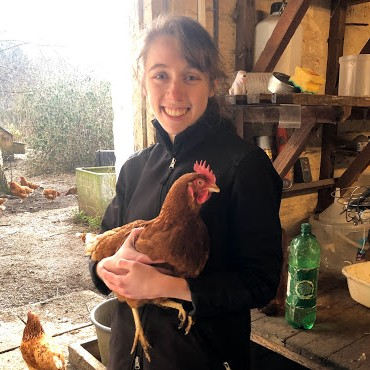
\includegraphics[width=0.5\textwidth]{../Images/chicken.jpg}

\vspace{1cm}
\end{frame}

\begin{frame}
	\Huge \bfseries Questions?
\end{frame}

\begin{frame}
\frametitle{References}
\footnotesize
Shapiro, L., Whitehead, S. A., \& Thomas, M. B. (2017). Quantifying the effects of temperature on mosquito and parasite traits that determine the transmission potential of human malaria. PLoS biology, 15(10), e2003489. 

\vspace{0.5cm}
Wang, J. Ogden, N.H., \& Zhu, H. (2011). The Impact of Weather Conditions on Culex pipiens and Culex restuans (Diptera: Culicidae) Abundance: A Case Study in Peel Region. Journal of Medical Entomology, 48(2), pages 468-475


\end{frame}

\end{document}

